
\documentclass[11pt, journal]{IEEEtran}


\usepackage{graphicx}


%% this is to get centered captions (figure)
\makeatletter
\long\def\@makecaption#1#2{\ifx\@captype\@IEEEtablestring%
\footnotesize\begin{center}{\normalfont\footnotesize #1}\\
{\normalfont\footnotesize\scshape #2}\end{center}%
\@IEEEtablecaptionsepspace
\else
\@IEEEfigurecaptionsepspace
\setbox\@tempboxa\hbox{\normalfont\footnotesize {#1.}~~ #2}%
\ifdim \wd\@tempboxa >\hsize%
\setbox\@tempboxa\hbox{\normalfont\footnotesize {#1.}~~ }%
\parbox[t]{\hsize}{\normalfont\footnotesize \noindent\unhbox\@tempboxa#2}%
\else
\hbox to\hsize{\normalfont\footnotesize\hfil\box\@tempboxa\hfil}\fi\fi}
\makeatother



% *** CITATION PACKAGES ***
%
\usepackage{cite}



% *** GRAPHICS RELATED PACKAGES ***
%
\ifCLASSINFOpdf
  \usepackage{graphicx}

\else

\fi



% *** SUBFIGURE PACKAGES ***
\usepackage[tight,footnotesize]{subfigure}


% *** PDF, URL AND HYPERLINK PACKAGES ***
%
\usepackage{url}


% correct bad hyphenation here
\hyphenation{op-tical net-works semi-conduc-tor}

\begin{document}
%
% paper title
% can use linebreaks \\ within to get better formatting as desired
\title{Analysis Of Ufo Sightings}


\author{ \parbox{3 in}{\centering Anna Bussas bussas@mail.hs-ulm.de\\
Sydney Nkemakolam nkemakolam@mail.hs-ulm.de\\
Kasparas Gudzius gudzius@mail.hs-ulm.de\\
Zhiwen Lian lian@mail.hs-ulm.de\\
Tim Hutttlestone huttlestone@mail.hs-ulm.de\\
				 University of Applied Sciences Ulm\\
 %        {\tt\small {goldstein}@hs-ulm.de}}
 }
}


% The paper headers
\markboth{ }{A Template Paper}




% make the title area
\maketitle

%%%%%%%%%%%%%%%%%%%%%%%%%%%%%%%%%%%%%%%%%%%%%%%%%%%%%%%%%%%%%%%%%%%%%%%%%%%%%%%%%%%%%%%%%%%%%%%%%%%%%%%%%%%%%%%%%%%%%%%%%%%%%%%%
%%%%%%%%%%%%%%%%%%%%%%%%%%%%%%%%%%%%%%%%%%%%%%%%%%%%%%%%%%%%%%%%%%%%%%%%%%%%%%%%%%%%%%%%%%%%%%%%%%%%%%%%%%%%%%%%%%%%%%%%%%%%%%%%
\begin{abstract}
Based on open data from kaggle.com and data processing based on the CRISP-DM model, it is observed that most people saw UFOs as a light shape in the US at night time during the Summer of 2011. 
\end{abstract}


%%%%%%%%%%%%%%%%%%%%%%%%%%%%%%%%%%%%%%%%%%%%%%%%%%%%%%%%%%%%%%%%%%%%%%%%%%%%%%%%%%%%%%%%%%%%%%%%%%%%%%%%%%%%%%%%%%%%%%%%%%%%%%%%
%%%%%%%%%%%%%%%%%%%%%%%%%%%%%%%%%%%%%%%%%%%%%%%%%%%%%%%%%%%%%%%%%%%%%%%%%%%%%%%%%%%%%%%%%%%%%%%%%%%%%%%%%%%%%%%%%%%%%%%%%%%%%%%%
\section{Introduction}
\label{sec:intro}
We intend to analyze the "Ufo Sightings" database from
the website kaggle.com to figure out when and where the UFOs show up mostly, and what they look like. 
\subsection{Scenario} \label{subsec:scenario}
The data source has in total 11 columns covering the sighting time, location, shape, duration and so on. As our goal is to find out the shapes, country and the number of ufo sightings depending on the time of day -daytime or nighttime-, we need to create a data warehouse containing the appropriate dimensions - Location, Time, etc.

\subsection{Structure of the Paper} \label{subsec:struct}
The paper is structured as follows: in Section~\ref{sec:dataunderstanding} we present the availability of Open Data we used in this project.
Then, in Section~\ref{sec:concept} we describe the adaptation of the original data to our expected data. Finally, we conclude our work in Section~\ref{sec:concl} with (XXXXXXXXXX placeholder --> to see if any section we want to add).
In Section ~\ref{sec:dataPreparation}, ~\ref{sec:modeling},~\ref{sec:Evaluation}, we will introduce data processing under CRISP-DM.


%%%%%%%%%%%%%%%%%%%%%%%%%%%%%%%%%%%%%%%%%%%%%%%%%%%%%%%%%%%%%%%%%%%%%%%%%%%%%%%%%%%%%%%%%%%%%%%%%%%%%%%%%%%%%%%%%%%%%%%%%%%%%%%%
\section{Open Data: UFO Sightings} \label{sec:dataunderstanding}
As part of the \emph{Data Understanding} phase for our data warehousing project, we first look at the state concerning our problem. The material presented in this section is based on Kaggle \cite{kaggle}.

%%%%%%%%%%%%%%%%%%%%%%%%%%%%%%%%%%%%%%%%%%%%%%%%%%%%%%%%%%%%%%%%%%%%%%%%%%%%%%%%%%%%%%%%%%%%%%%%%%%%%%%%%%%%%%%%%%%%%%%%%%%%%%%%
\section{Concept for Problem} \label{sec:concept}
During the \emph{Data Understanding} phase, we realized we didn't have out of the box columns containing some needed data. Additionally, some entries contained NULL values. Accordingly, there was need to have our Data prepared before the Analysis.

\subsection{Data Profiling}\label{subsec:dataProfiling}
In the \emph{Data Profiling} step, we discovered irrelevant columns in our dataset and hence had to drop them.  Accordingly, we agreed to only keep the following columns:
\begin{itemize}
    \item datetime
    \item city
    \item state
    \item country
    \item shape
    \item duration(second)
    \item date posted
\end{itemize}
Also, for the NULL values, we filled a necessary value in the corresponding columns using the below approach:
\begin{itemize}
    \item city / state / country\\
    If there are NULL values in city or state but not country, We will fill in the country value in those columns since our analysis on the location dimension will be based on the Country table as it's finest granularity. For those with both state and country missing, we will try to perform a string search on the city for some clue, find the country and manually map as accurately as possible. The rest without enough information were filled with "unknown".
    \item shape\\
    We will fill in "unknown" to replace the NULL values.
\end{itemize}

\subsection{Tools}\label{subsec:tools}
The summary of all tools used in this project and the application area:  
\begin{itemize}
    \item SQLiteManager\\
    Data Cleaning, ETL process, CDWH \& DM creation
    \item DBSchema\\
    Forward Engineering
    \item BIRT and MySql Workbench\\
    Analytics
    \item Python and Pandas\\
    Extra Data Cleaning and Enrichment
\end{itemize}
    
\subsection{DWH layout}\label{subsec:DWHLayout}
After the ETL process, we had a DHW which looks like this:
\begin{figure}[htb]
	\centering
		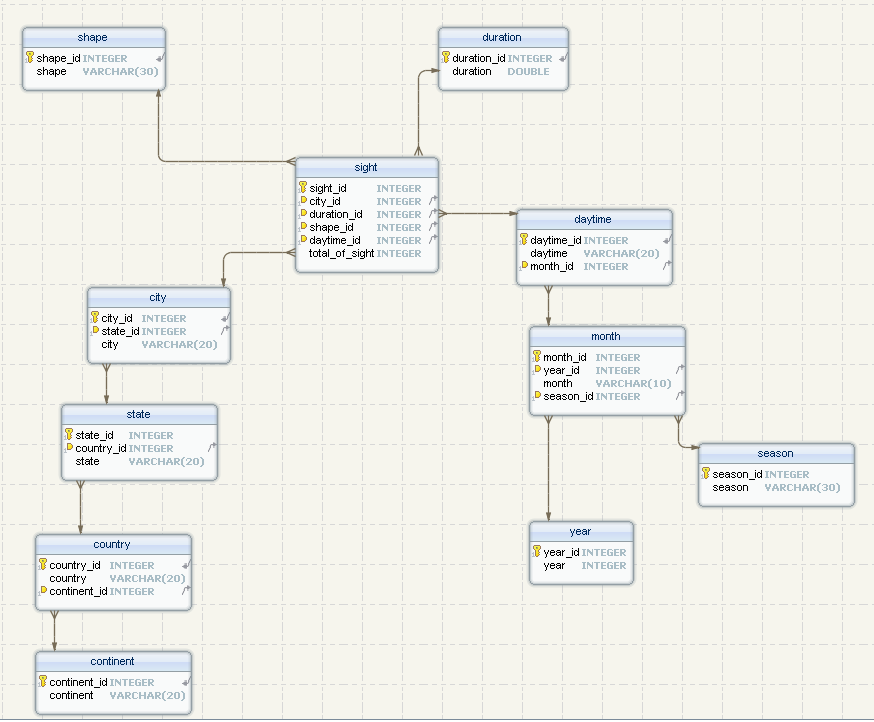
\includegraphics[width=1.0\columnwidth]{images/CDWHUFO}
	\caption{DWH layout}
	\label{fig:CDWHlayout}
\end{figure}

 
%%%%%%%%%%%%%%%%%%%%%%%%%%%%%%%%%%%%%%%%%%%%%%%%%%%%%%%%%%%%%%%%%%%%%%%%%%%%%%%%%%%%%%%%%%%%%%%%%%%%%%%%%%%%%%%%%%%%%%%%%%%%%%%%
%%%%%%%%%%%%%%%%%%%%%%%%%%%%%%%%%%%%%%%%%%%%%%%%%%%%%%%%%%%%%%%%%%%%%%%%%%%%%%%%%%%%%%%%%%%%%%%%%%%%%%%%%%%%%%%%%%%%%%%%%%%%%%%%
\section{Data Preparation} \label{sec:dataPreparation}
This section deals with the implementation of the concept described in Section~\ref{sec:concept} following the \emph{Data Preparation}
phase of CRISP-DM. 

To solve the problem, we took the following steps:
\begin{itemize}
  \item step 1 Extract \\
  Download the dataset from the website then create a database to store all raw data.
  \item step 2 Filtering\\
  Fill in values by the rule mentioned in \ref{subsec:dataProfiling}.
  \item step 3 Enrichment\\
  We would like to see some relationship between the sighting, season, daytime or nighttime, country and so on. In other words, we need different dimensions. So here "new" data is created by applying algorithms:
  \begin{itemize}
      \item Create new columns for the year, month, day, hour, daytime, season
      \item Column year, month, day, hour\\
      Extract data from column datetime
      \item Column daytime\\
      From 6am to 6pm is defined as daytime. The rest is defined as nighttime
      \item Column season\\
      Compute by aggregating corresponding seasonal months from the "month" column
  \end{itemize}
  
\end{itemize}

%%%%%%%%%%%%%%%%%%%%%%%%%%%%%%%%%%%%%%%%%%%%%%%%%%%%%%%%%%%%%%%%%%%%%%%%%%%%%%%%%%%%%%%%%%%%%%%%%%%%%%%%%%%%%%%%%%%%%%%%%%%%%%%%
\section{Modeling} \label{sec:modeling}
This section is to analyze the data we have prepared from Section ~\ref{sec:dataPreparation}.

To analyze, we took the following steps:
\begin{itemize}
    \item step 1\\
    Import Cleansed Data into DWH (see DWH Layout in ~\ref{subsec:DWHLayout})
    \item step 2\\
    For improved performance and speed during analysis, we created four data marts suiting our analytic goals (See Fig. \ref{fig:dm-cms}, \ref{fig:dm-css}, \ref{fig:dm-dcd}, \ref{fig:dm-scy})
      
    \begin{figure}[htb]
        \centering
            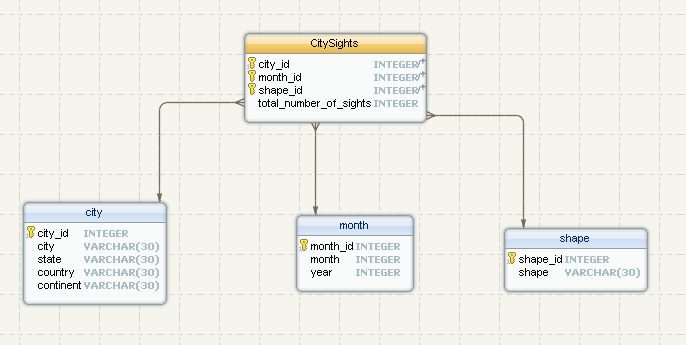
\includegraphics[width=1.0\columnwidth]{images/city-month-shape}
        \caption{Data mart - city/month/shape}
        \label{fig:dm-cms}
    \end{figure}

     \begin{figure}[htb]
            \centering
	            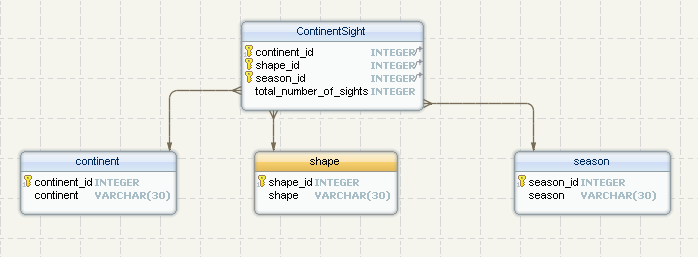
\includegraphics[width=1.0\columnwidth]{images/continent-shape-season}
            \caption{Data mart - continent/shape/season}
            \label{fig:dm-css}
        \end{figure}

     \begin{figure}[htb]
        \centering
            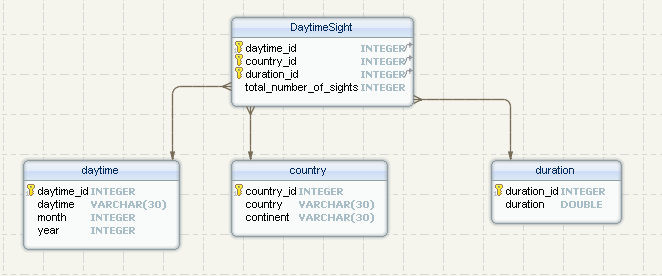
\includegraphics[width=1.0\columnwidth]{images/daytime-country-duration}
        \caption{Data mart - daytime/country/duration}
        \label{fig:dm-dcd}
    \end{figure}

     \begin{figure}[htb]
        \centering
            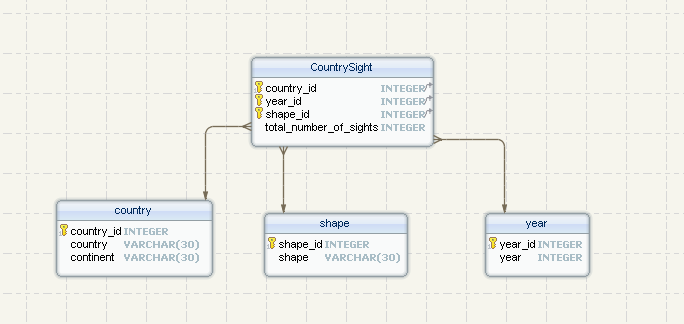
\includegraphics[width=1.0\columnwidth]{images/shape-country-year}
        \caption{Data mart - shape/country/year}
        \label{fig:dm-scy}
    \end{figure}
        
    \item step 3
    Using BIRT connected to the MySql-Workbench backend, we generated reports and found the following facts:
        \begin{itemize}
            \item Number of sightings in North America is extremely higher than in other continents. The next continent with the highest number of sightings is Europe,while there were no records for Africa, South America and Antarctica.(See Fig.\ref{fig:continent})\\
            - Data mart - Shape/Country/Year\\
            - Data cube - continent
                
            \item Nearly all sightings were in the US.(See Fig. \ref{fig:country})\\
            - Data mart - Shape/Country/Year\\
            - Data cube - contry
               
            \item The most Sightings were seen in 2011. We can see that it obviously increased between the years 1995 and 2011.(See Fig. \ref{fig:year} )\\
            - Data mart - Shape/Country/Year\\
            - Data cube - year
                
            \item UFOs were most seen during the Summer. (See Fig. \ref{fig:sight-season})\\
            - Data set - data mart - Continent/Shape/Season\\
            - Data cube - season
                 
            \item Different UFO shapes were recorded and the most common were "light-shaped".(See Fig. \ref{fig:shape})\\
            - Data set - data mart - Continent/Shape/Season\\
            - Data cube - shape
                
            \item In different continents, the most seen shape was also light. (See Fig. \ref{fig:shape-continent})\\
            - Data set - data mart - Continent/Shape/Season\\
            - Data cube - shape,continent
                
            \item In each season, light shape was also the most common. (See Fig. \ref{fig:shape-season})\\
            - Data set - data mart - Continent/shape/season\\
            - Data cube - season, shape
                
        \end{itemize}
        \begin{figure}[t]
            \centering
                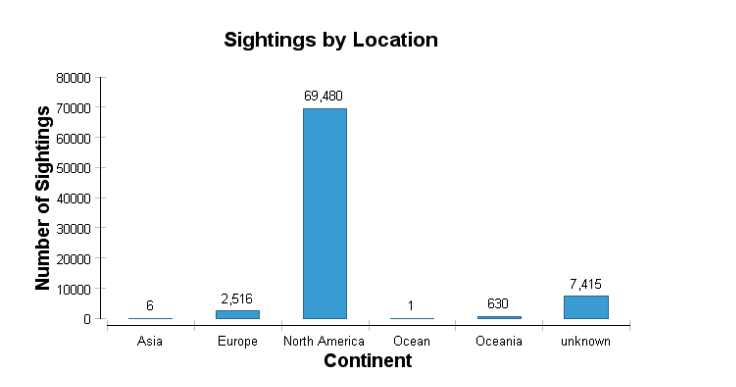
\includegraphics[width=1.0\columnwidth]{images/continent}
            \caption{Sightings by Location - Continent}
            \label{fig:continent}
        \end{figure}
        \begin{figure}[t]
            \centering
                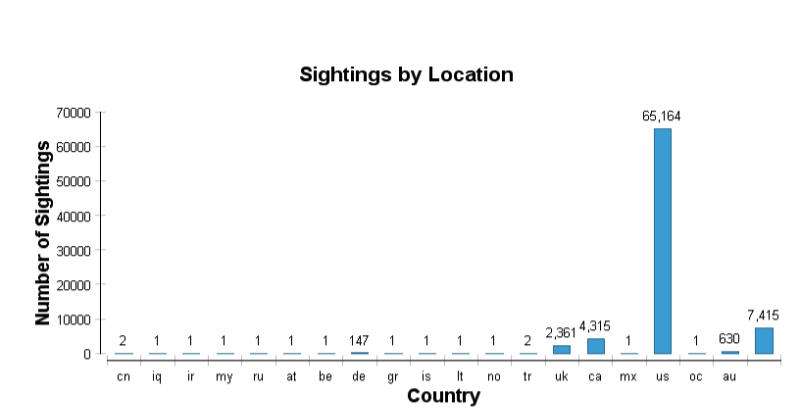
\includegraphics[width=1.0\columnwidth]{images/country}
            \caption{Sightings by Location - country}
            \label{fig:country}
        \end{figure}
        \begin{figure}[t]
            \centering
                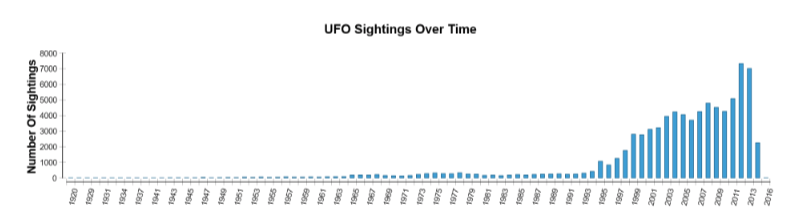
\includegraphics[width=1.0\columnwidth]{images/year}
            \caption{Sightings Over Time}
            \label{fig:year}
        \end{figure}
        \begin{figure}[t]
            \centering
                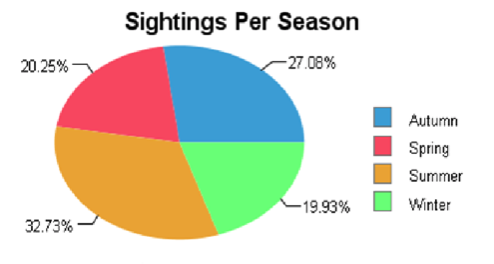
\includegraphics[width=1.0\columnwidth]{images/sightings-season}
            \caption{Sightings Per Season}
            \label{fig:sight-season}
        \end{figure}
        \begin{figure}[t]
            \centering
                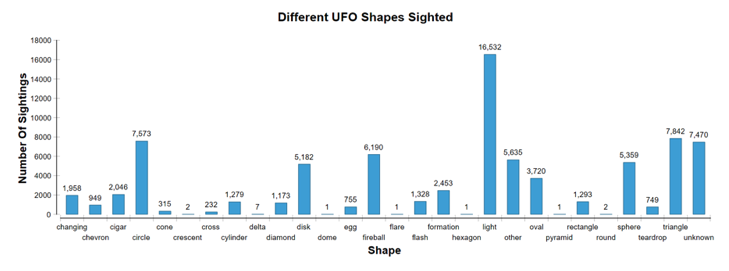
\includegraphics[width=1.0\columnwidth]{images/shape}
            \caption{Different UFO Shapes Sighted}
            \label{fig:shape}
        \end{figure}
        \begin{figure}[t]
            \centering
                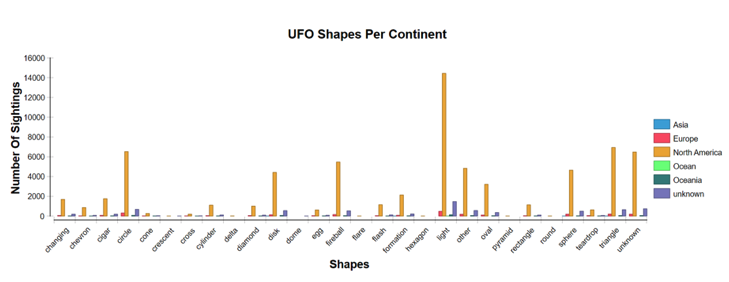
\includegraphics[width=1.0\columnwidth]{images/shape-continent}
            \caption{Shapes Per Continent}
            \label{fig:shape-continent}
        \end{figure}
        \begin{figure}[t]
            \centering
                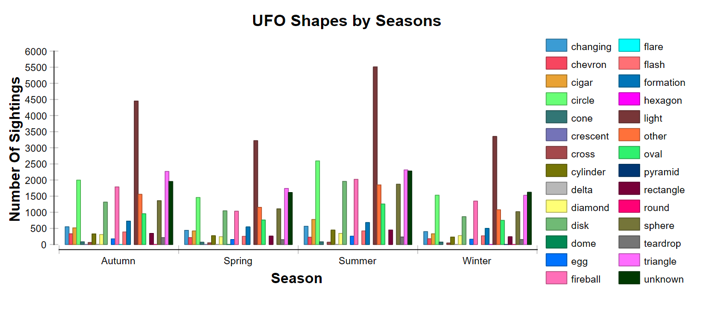
\includegraphics[width=1.0\columnwidth]{images/shapes-seasons}
            \caption{Shapes Per Seasons}
            \label{fig:shape-season}
        \end{figure}
\end{itemize}


%%%%%%%%%%%%%%%%%%%%%%%%%%%%%%%%%%%%%%%%%%%%%%%%%%%%%%%%%%%%%%%%%%%%%%%%%%%%%%%%%%%%%%%%%%%%%%%%%%%%%%%%%%%%%%%%%%%%%%%%%%%%%%%%
\section{Evaluation} \label{sec:Evaluation}
From the reports, we can see the rendered facts on Ufo shapes, country of sighting, and sightings depending on season and daytime -day or night, as well as reports in different dimensions. We can safely say that we have reached the project goals after evaluation.

%%%%%%%%%%%%%%%%%%%%%%%%%%%%%%%%%%%%%%%%%%%%%%%%%%%%%%%%%%%%%%%%%%%%%%%%%%%%%%%%%%%%%%%%%%%%%%%%%%%%%%%%%%%%%%%%%%%%%%%%%%%%%%%%
\section{Conclusion} \label{sec:concl}
In this paper, we have shown the process and technicalities applied in building a CDWH and appropriate Data marts following the CRISP-DM process to facilitate analysis and proper visualization of the different dimensions in the Ufo Database which contains recorded Ufo sightings spanning a period of about One century.

%%%%%%%%%%%%%%%%%%%%%%%%%%%%%%%%%%%%%%%%%%%%%%%%%%%%%%%%%%%%%%%%%%%%%%%%%%%%%%%%%%%%%%%%%%%%%%%%%%%%%%%%%%%%%%%%%%%%%%%%%%%%%%%%
%%%%%%%%%%%%%%%%%%%%%%%%%%%%%%%%%%%%%%%%%%%%%%%%%%%%%%%%%%%%%%%%%%%%%%%%%%%%%%%%%%%%%%%%%%%%%%%%%%%%%%%%%%%%%%%%%%%%%%%%%%%%%%%%
% see file Literatur/bibliography!
\bibliographystyle{plaindin}
\bibliography{bibliography}

\end{document}
